\documentclass{article}
\usepackage[utf8]{inputenc}
\usepackage[portuges]{babel}
\usepackage{ntheorem}
\usepackage{amsfonts}
\usepackage{amsmath}
\usepackage{amssymb}
\usepackage{diffcoeff}

%\usepackage[margin=1.5in]{geometry}
\usepackage{multicol}
\theorembodyfont{\upshape}
\theoremseparator{.}
\newtheorem{ex}{Exercício}

\usepackage{enumitem}
\setlist[enumerate, 1]{label=\alph*)}

\usepackage{listings}
\lstset{basicstyle=\ttfamily,mathescape,keepspaces,tabsize=2,
literate=
  {á}{{\'a}}1
  {à}{{\`a}}1
  {ã}{{\~a}}1
  {é}{{\'e}}1
  {ê}{{\^e}}1
  {í}{{\'i}}1
  {ó}{{\'o}}1
  {ú}{{\'u}}1
  {ç}{{\c{c}}}1}
\usepackage{graphicx}
\usepackage{url}
\usepackage{hyperref}

\title{Mini-Projetos de ME}
\author{}
\date{}
\setlength{\parindent}{0pt}
\newcommand{\Z}{\mathbb{Z}}
\newcommand{\R}{\mathbb{R}}
\newcommand{\N}{\mathbb{N}}
\newcommand{\Q}{\mathbb{Q}}


\newcommand{\T}{\mathbb{T}}

\begin{document}

\section{Baralhos}

Neste exercício vai investigar formas de baralhar baralhos de cartas. Para este efeito, o conteúdo das cartas é irrelevante, pelo que basta representar as cartas por números de 1 a 52.

\begin{ex}
Considere o seguinte algoritmo para baralhar um baralho.

Um `riffle shuffle' consiste em partir o baralho ao meio e juntar as duas metades com as cartas a alternar. Por exemplo, dado um baralho cujas cartas são $c_1, c_2, \dots, c_{2n}$, o seu riffle shuffle é dado por
\[c_1, c_{n+1}, c_2, c_{n+2}, \dots, c_n, c_{2n}.\]

Se o baralho de cartas tiver um número ímpar de cartas, digamos $c_1, \dots, c_{2n+1}$, o seu riffle shuffle é dado por
\[c_1, c_{n+2}, \dots, c_n, c_{2n-1}, c_{n+1}.\]

Implemente uma função que recebe um baralho de cartas (ou seja, uma lista) e retorna o seu riffle shuffle. Os seguintes comandos poderão ser úteis: \texttt{Join}, \texttt{Riffle}.
\end{ex}

\begin{ex}
Apresentamos na figura \ref{shuffle8} uma visualização dos diversos riffle shuffles de um baralho de oito cartas, isto é: a $n$-ésima linha representa o baralho após $n$ riffle shuffles.

Como pode ver, após três shuffles o baralho volta à situação original. A figura \ref{shuffle52} mostra também o resultado de aplicar o riffle shuffle a um baralho de 52 cartas, e como pode perceber pela figura, o baralho volta à posição original após 8 shuffles.

Verifique estas afirmações. O comando \texttt{Nest} poderá ser útil.

\begin{figure}
\centering
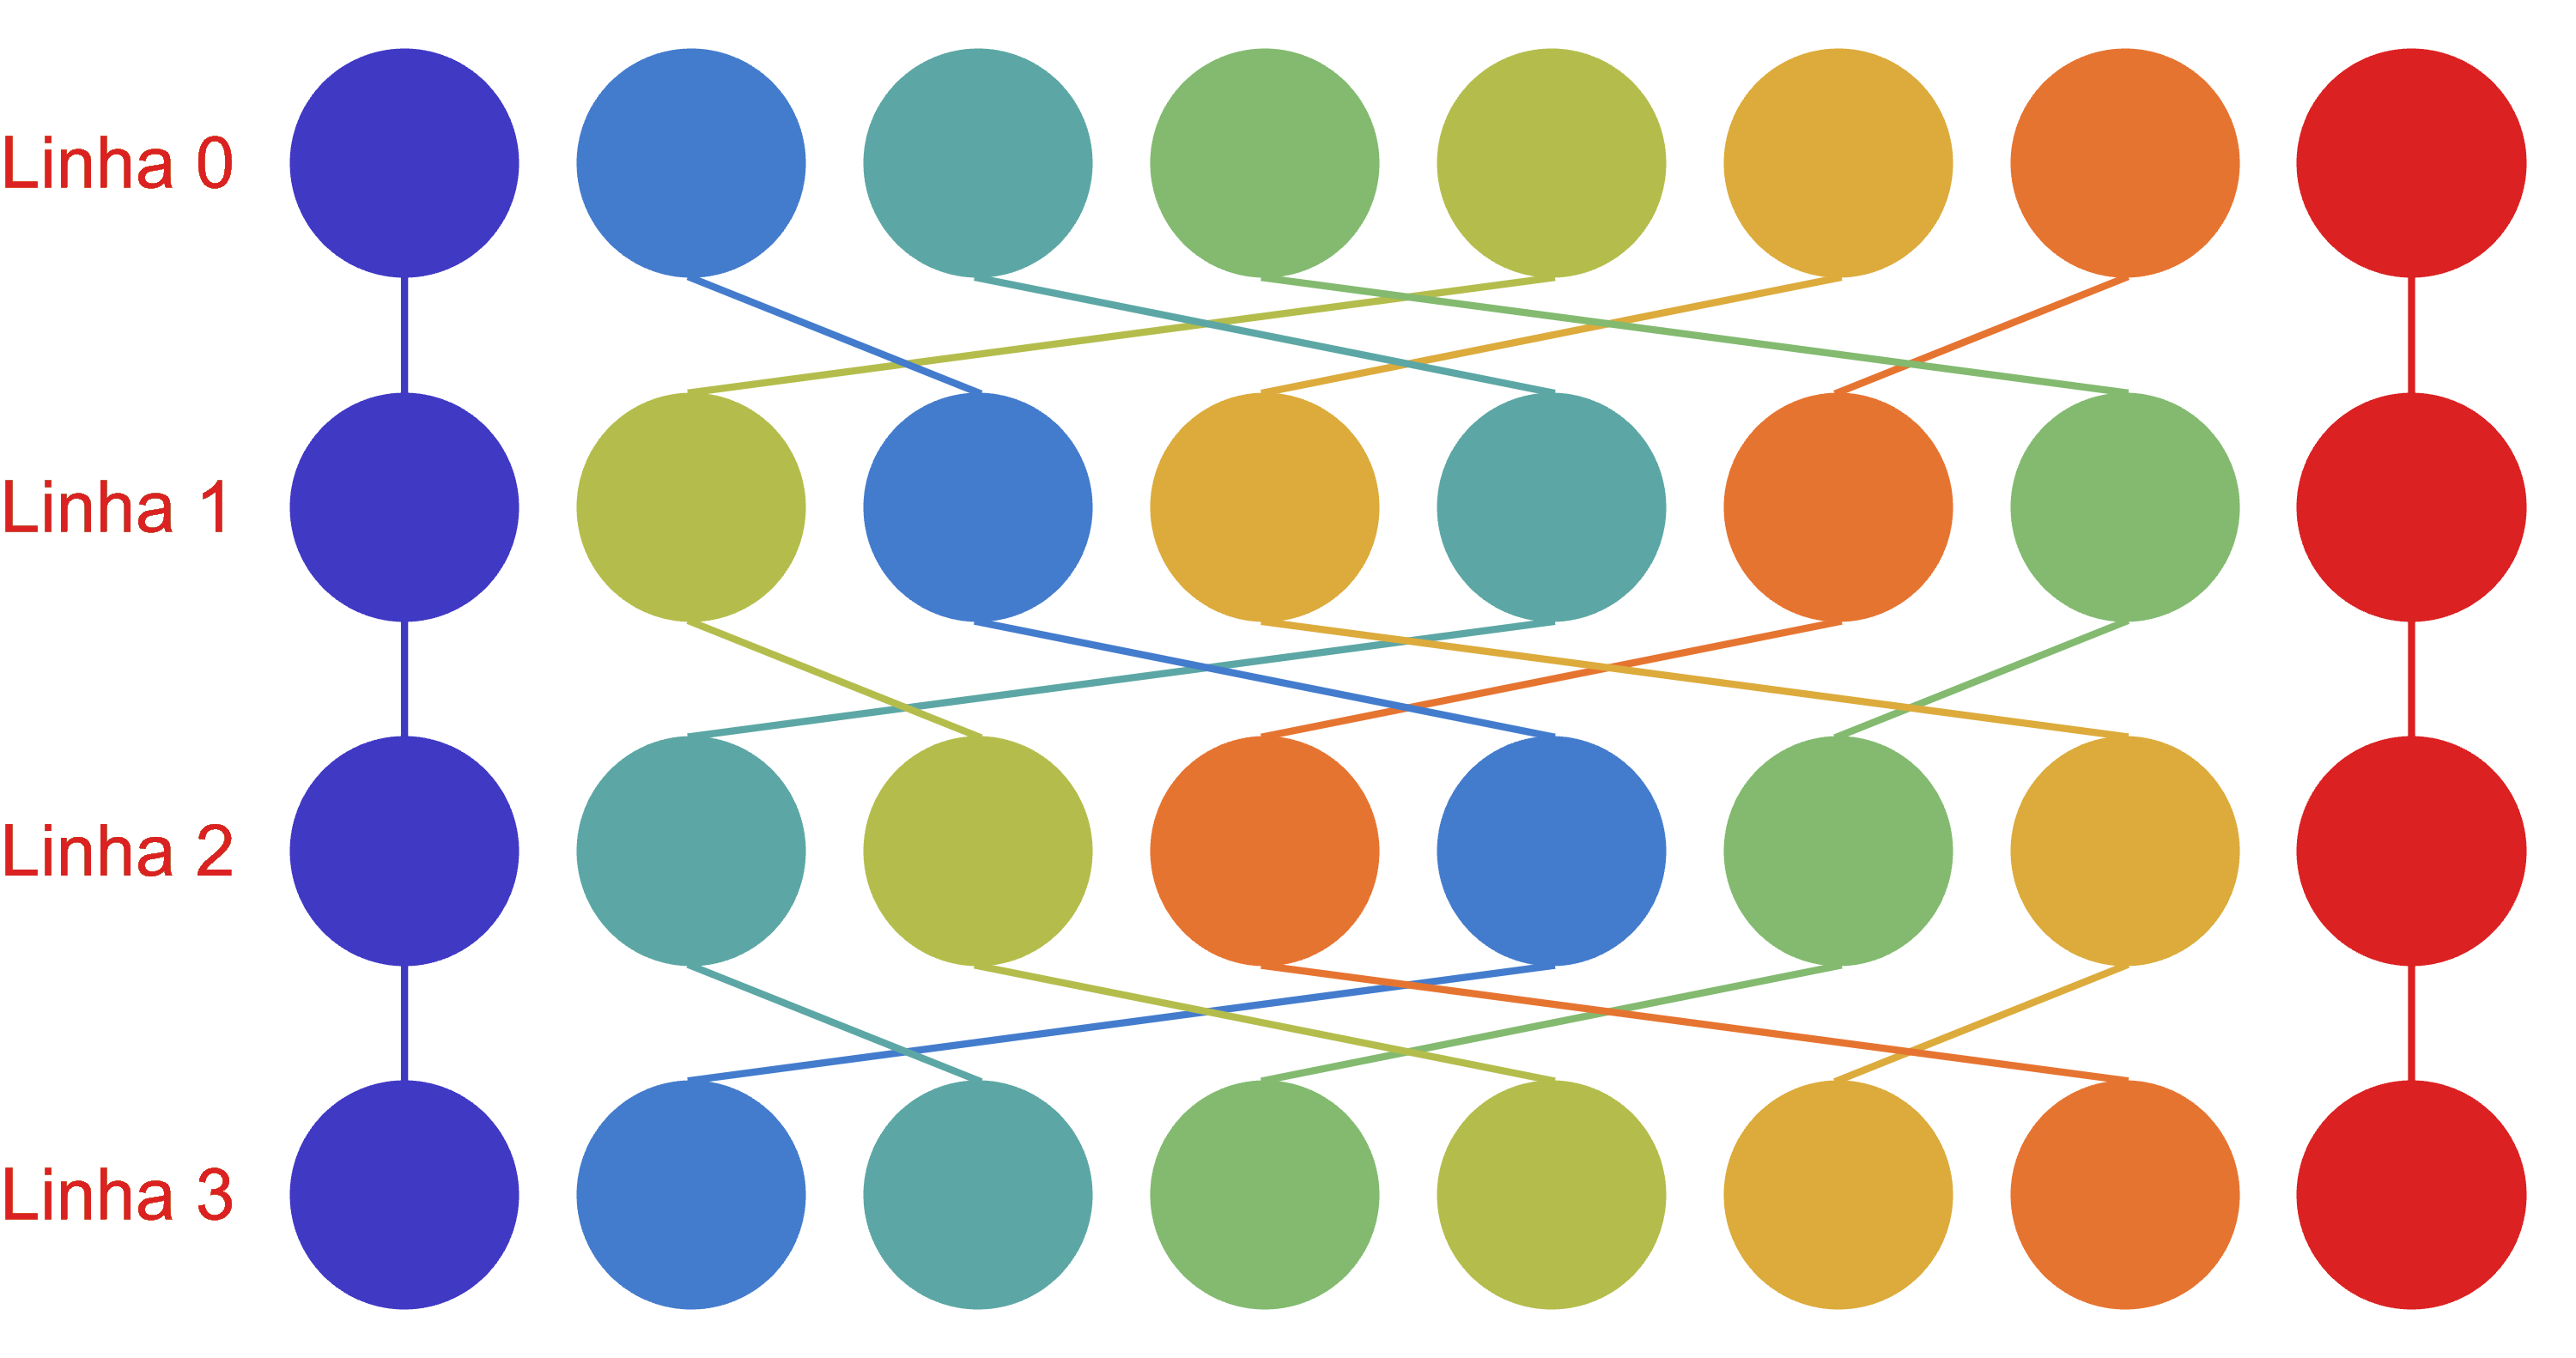
\includegraphics[width=.75\textwidth]{shuffle8}
\caption{Uma visualização das iterações do riffle shuffle num baralho com 8 cartas.}\label{shuffle8}
\end{figure}

\begin{figure}
\centering
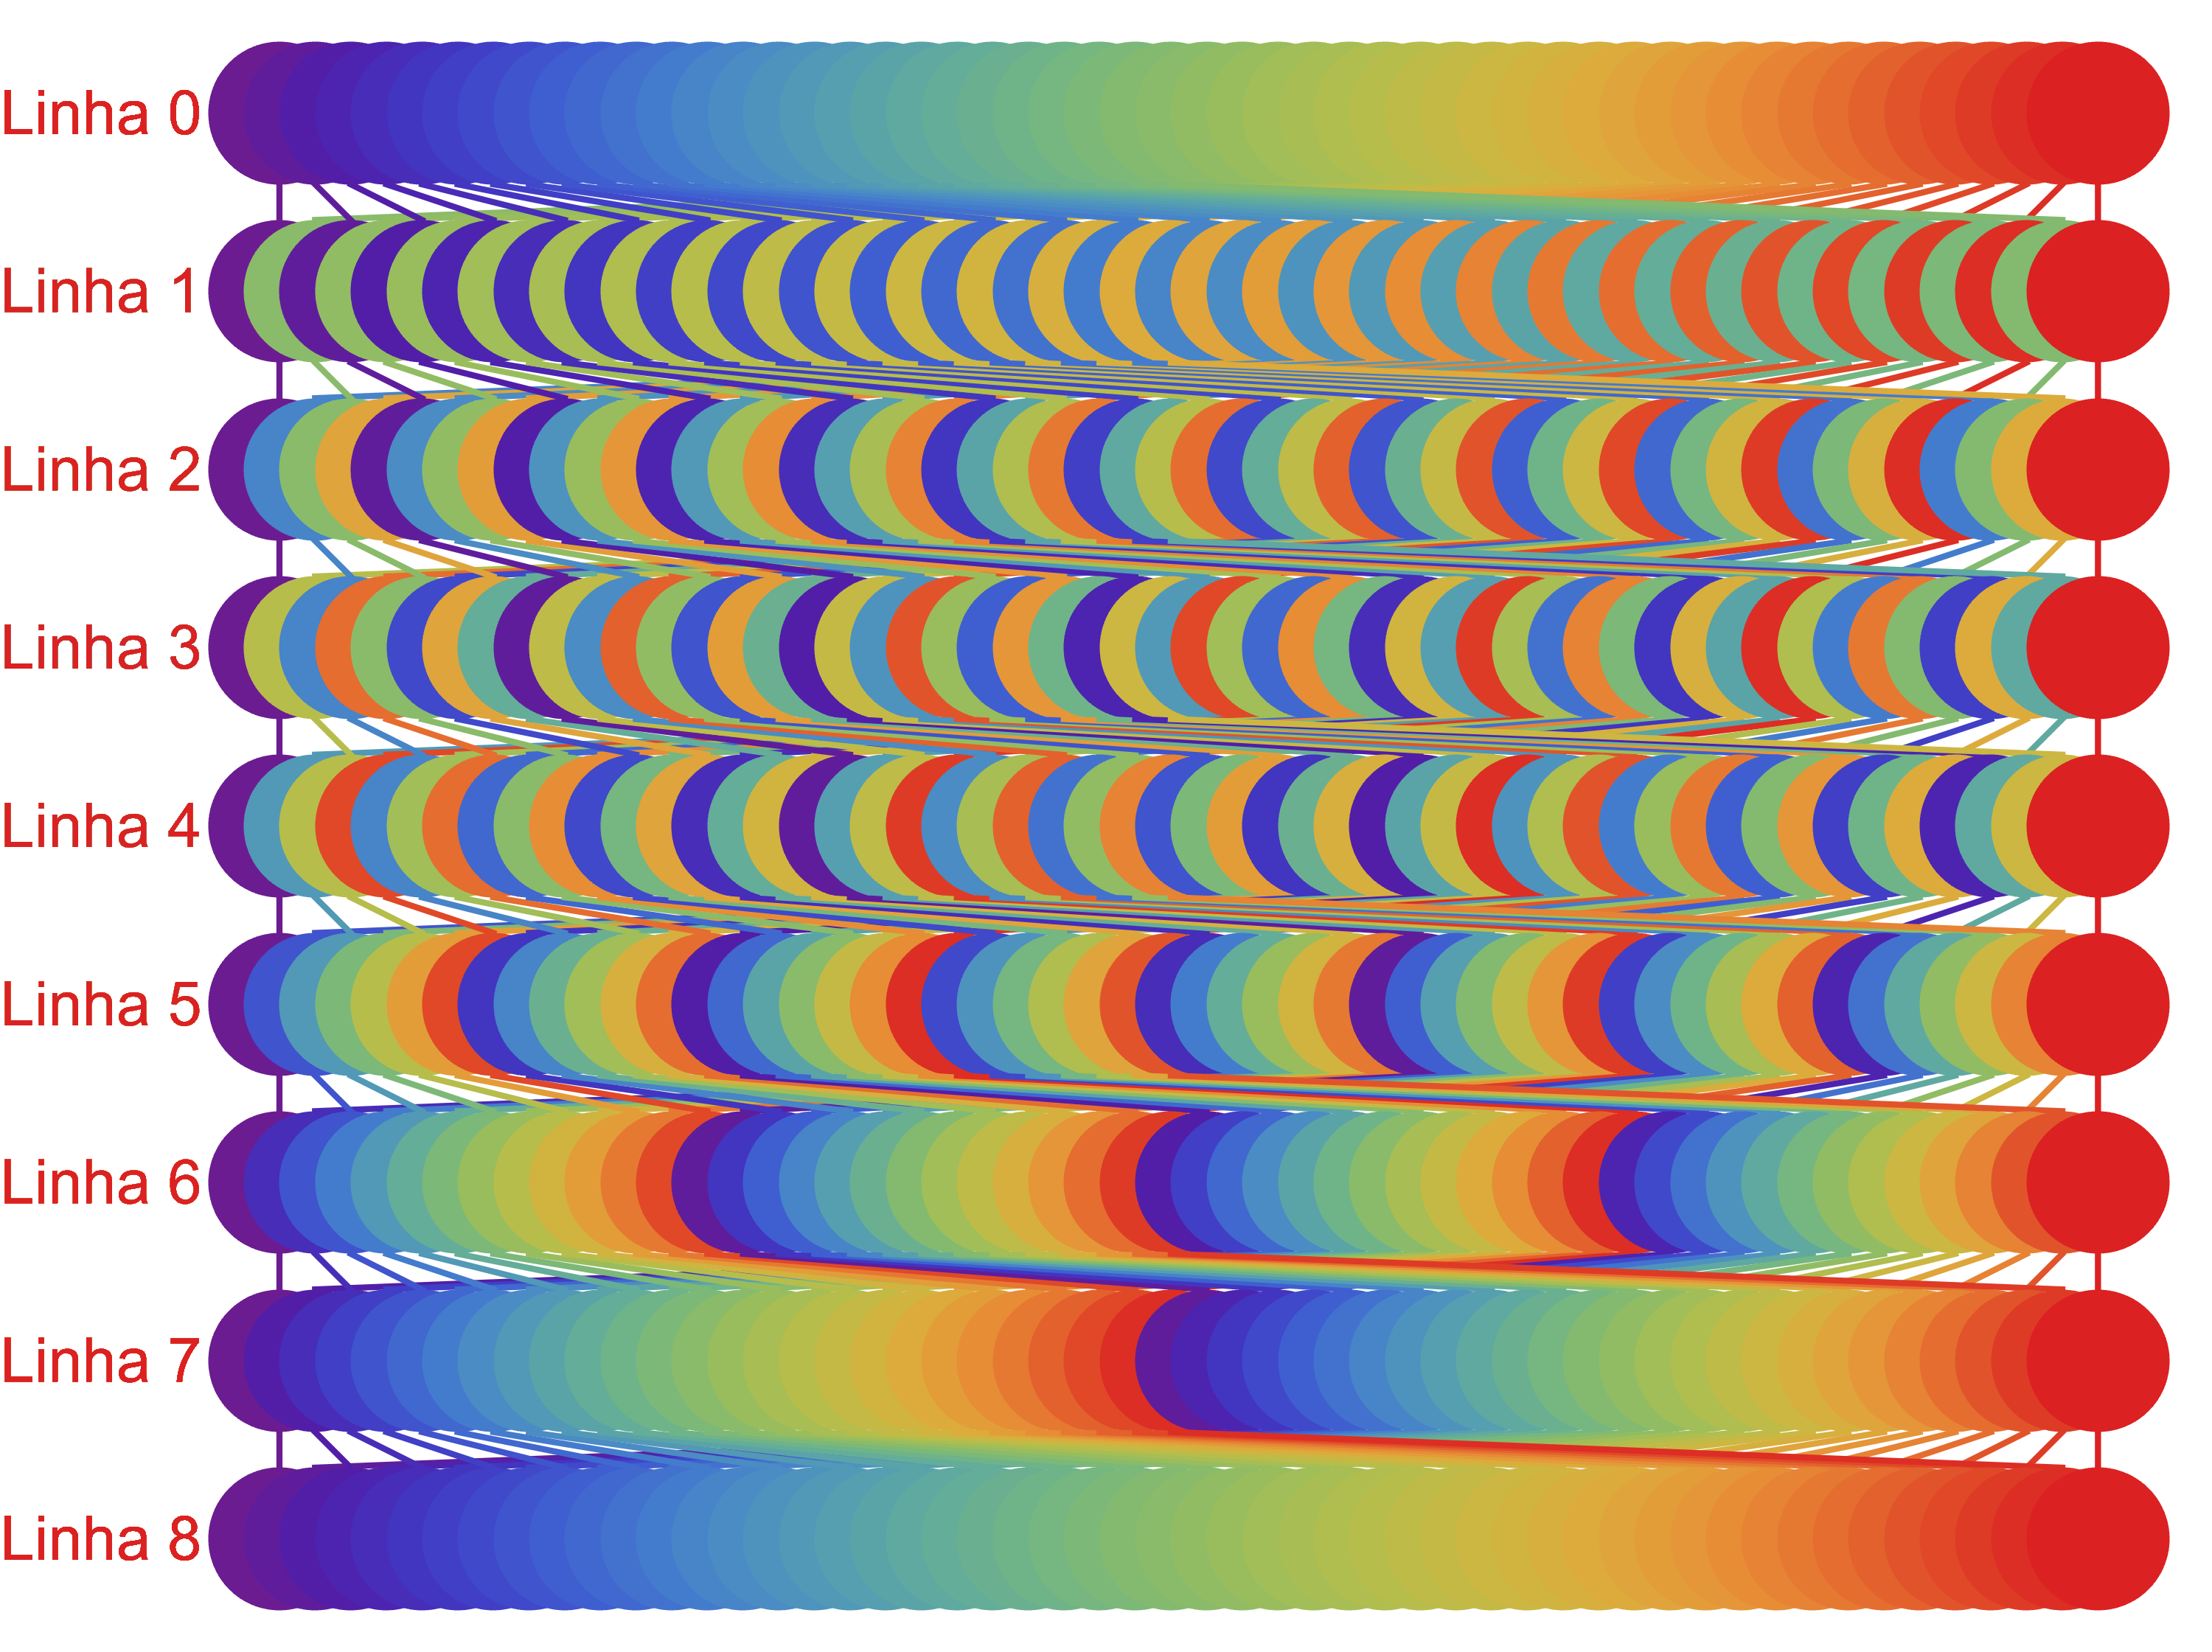
\includegraphics[width=.75\textwidth]{shuffle52}
\caption{Oito riffle shuffles de um baralho com 52 cartas.}\label{shuffle52}
\end{figure}
\end{ex}

\begin{ex}
Defina uma função $ord$ (que, dado $n$, retorna o número de riffle shuffles necessários para um baralho com $n$ cartas retornar à posição original.

Use a função \texttt{DiscretePlot} para mostrar o gráfico dessa função para alguns valores de $n$. Use esse gráfico para formular uma conjetura que relacione os valores de $ord(n)$ para $n$ par e ímpar.
\end{ex}

\begin{ex}
Faça um gráfico de $ord(n)$ apenas com valores pares de $n$. Usando a função \texttt{Show}, sobreponha a este os gráficos de $y = x-2$ e $y = \frac{\log x}{\log2}$.

Formule uma conjetura que relacione estas três funções.
\end{ex}

\begin{ex}
Investigue os valores pares de $n$ tais que $ord(n) = \frac{\log x}{\log 2}$. Quais são estes valores?
\end{ex}

\begin{ex}
Difícil: Elabore uma forma de visualizar estes embaralhamentos, de modo a criar figuras como a figura \ref{shuffle8} e a figura \ref{shuffle52}.
\end{ex}

\end{document}